\chapter{Filtrage des graphes}
\section{Introduction}
Le filtrage des graphes est l'une des caractéristiques essentielles que tout système d'analyse des graphes devrait pouvoir fournir, car il ouvre les portes à de nombreuses applications, pour n'en citer que quelques-unes, un analyste de données pourrait vouloir éliminer toutes les valeurs extrêmes qui peuvent influencer l'exactitude de ses résultats.\\
Mon but pendant le stage était d'ajouter des capacités de filtrage supplémentaires, alors que la plupart des infrastructures étaient déjà fournies pour moi, en particulier ce que je devais faire est d'utiliser ces infrastructures de la bonne manière pour atteindre mon objectif.\\
PGX.D prenait déjà en charge les filtres basés sur des expressions de filtrage, mais il manquait de nombreuses autres possibilités capabilités, comme le filtrage basé sur une collection ou un result-set.\\
Dans la suite de ce chapitre, je me concentrerai sur deux types de filtres que j'ai mis en œuvre, le premier consiste à créer un sous-graphe basé sur une collection, et le second consiste en l'opération inverse, c'est-à-dire créer une collection basée sur un filtre de sous-graphe, et à la fin, je présenterai certains des efforts que j'ai faits pour mettre en œuvre le filtrage basé sur un result-set.\\

\section{Conception du filtrage des graphes en mode distribué (général).}
Le flux d'évaluation d'un filtre en PGX.D peut se modéliser comme suit :
\begin{figure}[H]  
  \centering
    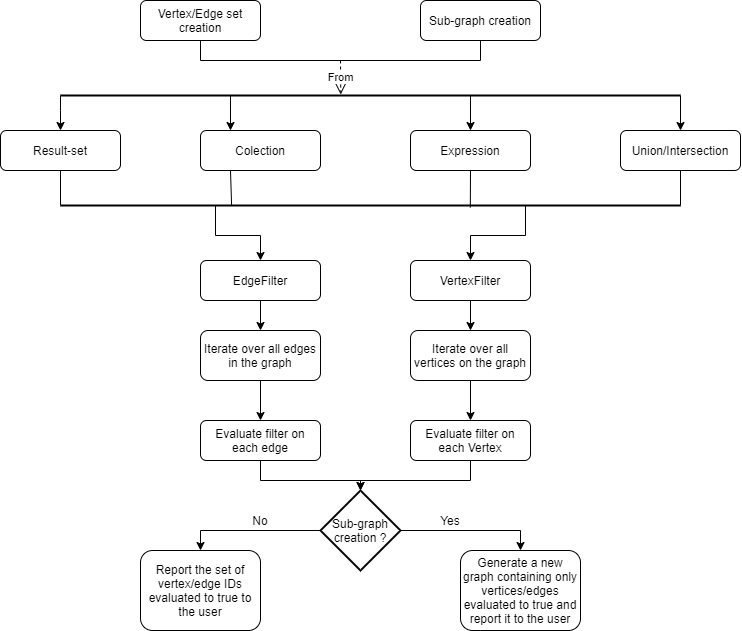
\includegraphics[width=1\textwidth]{chapitre3/Figures/Set-SubGraph-creation.png}
  \caption{Diagramme de flux de l'opération du filtrage}
\end{figure}

La création d'une collection de sommets/arêtes dans PGX peut se faire par plusieurs types de filtres :

\begin{itemize}[label=\textbullet]
\item  À partir d'un result-set : le résultat de l'exécution d'une requête PGQL.
\item  Une collection : Elle peut être générée manuellement ou à partir d'un filtre de sous-graphes (ce dont nous parlerons plus tard)
\item  Une expression : C'est une requête spéciale, qui est traduite en requête PGQL et ensuite exécutée.
\item  Une Union/Intersection : C'est le cas lorsque vous voulez appliquer plusieurs filtres à la fois.
\end{itemize}

Chacun de ces filtres peut être spécifié soit pour les arêtes, soit pour les sommets, et dans ce cas, il sera appelé VertexFilter ou EdgeFilter en fonction de la cible que nous spécifions dans notre requête.\\

\section{Le filtre est un VertexFilter(Filtre des sommets)}
Pour povoir filtrer un graphe par ces sommets, deux étapes essentielles sont nécessaires dans PGX:

\begin{enumerate}[label=\arabic*)]
\item  Pour chaque sommet du graphe, évaluez le filtre, placez un indicateur temporaire sur ce sommet, cette indicateur est un booléen qui précise si le sommet doit être conservé dans le sous-graph résultant, et nous envoyons le résultat de l'évaluation à tous les sommets entrants, ce qui réduit la quantité de messages à envoyer ("dans le cas où deux sommets ne se trouvent pas dans la même machine”):
\begin{figure}[H]  
  \centering
    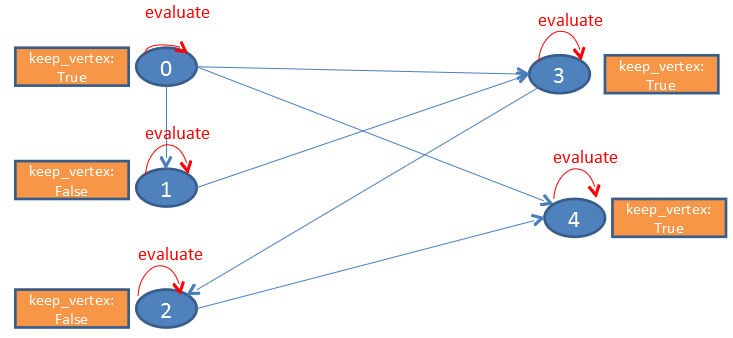
\includegraphics[width=1\textwidth]{chapitre3/Figures/VertexFilter1.png}
  \caption{1re étape de l'évaluation d'un filtre des sommets}
\end{figure}

\item  Chaque sommet ayant un bord sortant vers un autre sommet qui a été évalué comme vrai recevra un message de ce sommet pour potentiellement garder l'arête qui leur relié dans le cas où il serait évalué comme vrai.
\begin{figure}[H]  
  \centering
    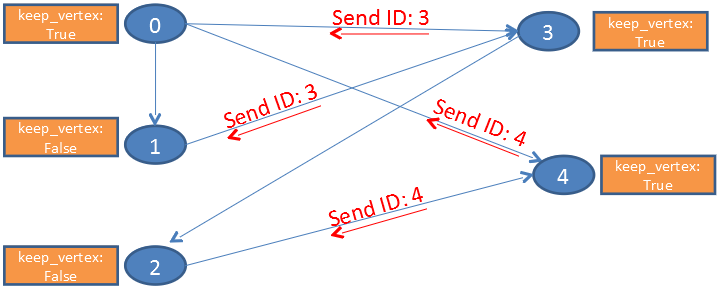
\includegraphics[width=1\textwidth]{chapitre3/Figures/VertexFilter2.png}
  \caption{2éme étape de l'évaluation d'un filtre des sommets}
\end{figure}
\end{enumerate}

\section{Le filtre est un EdgeFilter(Filtre des arêtes)}
Une arête est la composition de deux sommets (source, destination). Nous avons donc besoin d'informations sur les deux sommets pour pouvoir évaluer le filtre, ce qui implique plus d'étapes. Aussi il faut noter que l'évaluation du filtre ne se fait que sur la source de l'arête et non sur la destination :\\
\textbf{On à quatre étapes :}
\begin{enumerate}[label=\arabic*)]
\item  Envoyer les propriétés nécessaires à l'évaluation du filtre d'arête à la source (donc, à tous les voisins entrants de la destination), puisque les propriétés sont stockées dans les machines possédant le sommet
\begin{figure}[H]  
  \centering
    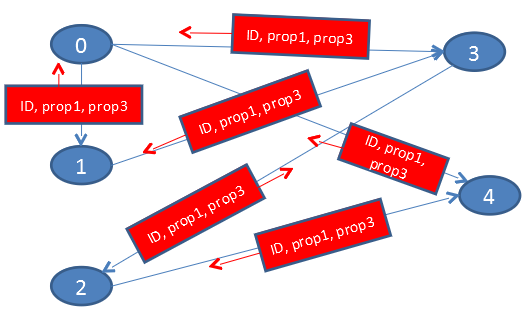
\includegraphics[width=0.8\textwidth]{chapitre3/Figures/EdgeFilter1.png}
  \caption{1er étape de l'évaluation d'un filtre des arêtes}
\end{figure}

\item  Pour chaque entrée de données de filtrage (propriétés, et ID de destination) arrivant des sommets de destination des arêtes sortantes du sommet source actuel :
    \begin{enumerate}[label=\alph*)]
    \item  Nous déterminons l'arête correspondante pointant vers la destination.
    \item  Nous évaluons le filtre à l'aide des données que nous avons reçues.
    \item  Si le filtre est évalué positivement, nous fixons un indicateur temporaire à la valeur "true" dans la source et l'arête évaluée.
    \item  Pour tous les sommets de destination, si le filtre est évalué positivement, envoyez un message qui indique que nous voulons le garder.
    \end{enumerate}
\begin{figure}[H]  
  \centering
    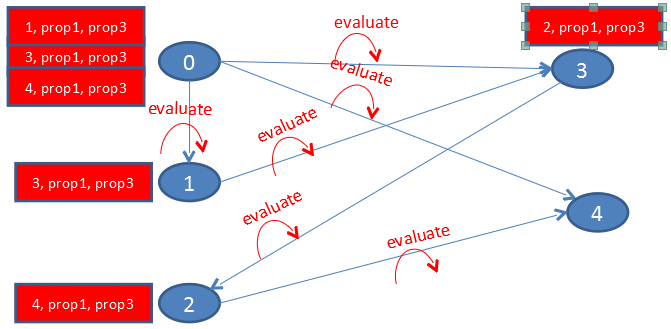
\includegraphics[width=1\textwidth]{chapitre3/Figures/EdgeFilter2.png}
  \caption{2éme étape de l'évaluation d'un filtre des sommets}
\end{figure}

\item  Lorsque le sommet de destination reçoit un message "keep", un indicateur est fixé à true pour garder le sommet.
\begin{figure}[H]
  \centering
    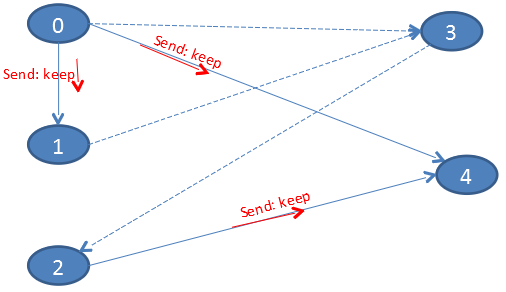
\includegraphics[width=1\textwidth]{chapitre3/Figures/EdgeFilter3.png}
  \caption{3éme étape de l'évaluation d'un filtre des arêtes}
\end{figure}

\item  Dernière étape (Étape commune entre le deux types de filtres EdgeFilter et VertexFilter ):
Nous parcourons tous les sommets/arêtes du graphe et si l'indicateur temporaire de à comme valeur "true", nous les ajoutons à un nouveau sous-graphe. Et enfin, nous communiquons le sous-graphe au client.
\end{enumerate}

\section{Conception de l'évaluation du filtrage (Filtre basé sur une collection)}
\subsection{Aperçu}
Une collection est un ensemble d'éléments homogènes, dans notre contexte, ces éléments sont les ID des sommets que nous voulons conserver dans le sous-graph résultant.\\
La création d'une collection peut se faire de plusieurs façons dans PGX (manuellement en utilisant l'API de la collection, en utilisant un algorithme ...etc.) pour présenter notre solution, nous utiliserons une collection construite manuellement pour filtrer un simple graphe.\\
À partir de cette collection, nous créons un filtre de sommet ou d'arête que nous appliquons sur le graphe original. En mode distribué, cela implique que la collection sera également distribuée, dans notre système, nous nous assurons que l'ID de chaque sommet, s'il est correct, est placé dans la sous-collection qui résidera dans la machine contenant ce sommet.\\

\begin{figure}[H]  
  \centering
    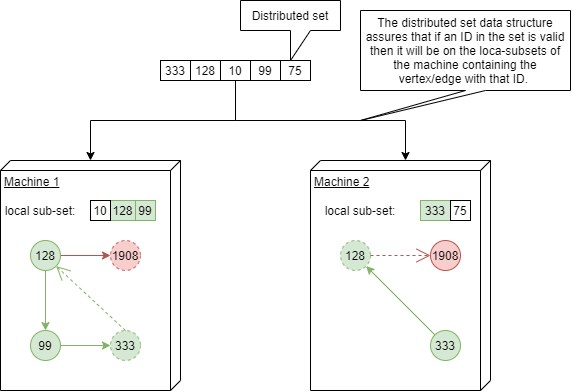
\includegraphics[width=1\textwidth]{chapitre3/Figures/SubgraphFromCollection.png}
  \caption{Exemple qui démontre l'exécution d'un filtre basé sur une collection}
\end{figure}

\subsection{Implémentation}
\begin{enumerate}[label=\arabic*)]
\item  On itère sur le graphe, sommet par sommet ou arête par arête selon le type de filtre.
\item  Nous vérifions si l'ID du sommet actuel est présent dans la collection locale ou non, s'il existe, le filtre l'évalue comme vrai et nous fixons l'indicateur pour garder le sommet ou l'arête comme nous l'avons décrit précédemment.
\end{enumerate}
Cela est fait de manière concurrente, mais comme nous ne faisons que lire, nous n'avons pas eu de problèmes de synchronisation.


\section{Conception de l'évaluation du filtrage (Création d’une collection à partir d’un filtre de sous graphe)}
Nous évaluons le filtre sur le graphe sans la dernière étape, en créant le nouveau sous-graph. Au lieu de cela, chaque fois qu'un sommet ou une arête est évalué comme vrai, nous l'ajoutons à une collection distribuée.\\
\begin{figure}[H]  
  \centering
    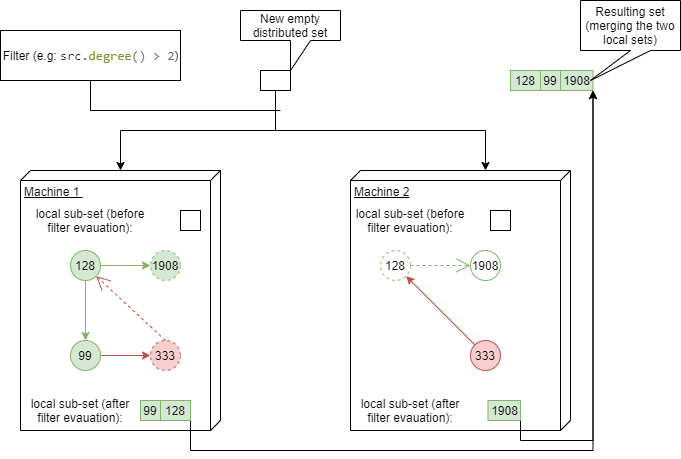
\includegraphics[width=1\textwidth]{chapitre3/Figures/CreateSetFromFilter.png}
  \caption{Exemple qui démontre l'extraction d'une collection à partir d'un autre filtre (basé sur une expression dans ce cas)}
\end{figure}